\documentclass[border=10pt]{standalone}
\usepackage{tikz}
\usepackage{amsmath}
\usetikzlibrary{arrows.meta, positioning, fit, backgrounds, calc, decorations.pathreplacing}

\newcommand{\groupbox}[6]{% #1=draw #2=fill #3,#4=lower-left #5,#6=upper-right
  \begin{scope}[on background layer]
    \draw[rounded corners=9pt, very thick, draw=#1, fill=#2] (#3,#4) rectangle (#5,#6);
  \end{scope}}

\begin{document}
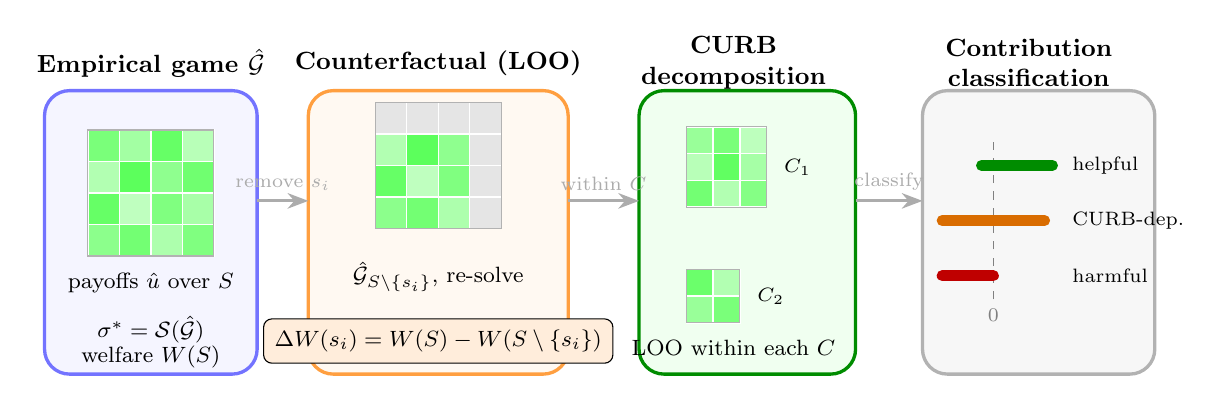
\begin{tikzpicture}[
  font=\small, >=Stealth,
  gtitle/.style={font=\bfseries\small, align=center},
  sub/.style={font=\footnotesize},
  tiny/.style={font=\scriptsize},
  flow/.style={->, thick, gray!65, line width=1pt},
]

% ---------- STAGE 1: EMPIRICAL GAME ----------
\begin{scope}[shift={(0,0)}]
  \foreach \cx/\cy/\g in {%
    0/0/45,0/1/60,0/2/30,0/3/52, 1/0/55,1/1/25,1/2/64,1/3/36,%
    2/0/32,2/1/50,2/2/44,2/3/60, 3/0/50,3/1/34,3/2/56,3/3/28}{%
    \fill[green!\g!white, draw=white, line width=0.5pt]
      (\cx*0.40,\cy*0.40) rectangle ++(0.40,0.40);}
  \draw[gray!60] (0,0) rectangle (1.6,1.6);
  \node[sub] at (0.8,-0.34) {payoffs $\hat{u}$ over $S$};
  \node[sub, anchor=north] at (0.8,-0.64) {$\sigma^*=\mathcal{S}(\hat{\mathcal{G}})$};
  \node[sub, anchor=north] at (0.8,-1.02) {welfare $W(S)$};
\end{scope}
\node[gtitle] at (0.8,2.45) {Empirical game $\hat{\mathcal{G}}$};
\groupbox{blue!55}{blue!4}{-0.55}{-1.5}{2.15}{2.1}

% ---------- STAGE 2: COUNTERFACTUAL LOO ----------
\begin{scope}[shift={(3.65,0.35)}]
  \foreach \cx/\cy/\g in {%
    0/0/45,0/1/60,0/2/30, 1/0/55,1/1/25,1/2/64, 2/0/32,2/1/50,2/2/44}{%
    \fill[green!\g!white, draw=white, line width=0.5pt]
      (\cx*0.40,\cy*0.40) rectangle ++(0.40,0.40);}
  \foreach \cx/\cy in {3/0,3/1,3/2,3/3,0/3,1/3,2/3}{%
    \fill[gray!20, draw=white, line width=0.5pt]
      (\cx*0.40,\cy*0.40) rectangle ++(0.40,0.40);}
  \draw[gray!60] (0,0) rectangle (1.6,1.6);
  \node[sub, anchor=north] at (0.8,-0.30) {$\hat{\mathcal{G}}_{S\setminus\{s_i\}}$, re-solve};
\end{scope}
\node[gtitle] at (4.45,2.45) {Counterfactual (LOO)};
\node[draw, rounded corners=3pt, fill=orange!14, sub, align=center, inner sep=4pt]
  at (4.45,-1.08) {$\Delta W(s_i)=W(S)-W(S\setminus\{s_i\})$};
\groupbox{orange!75}{orange!5}{2.8}{-1.5}{6.1}{2.1}

% ---------- STAGE 3: CURB DECOMPOSITION ----------
\begin{scope}[shift={(7.6,0)}]
  \begin{scope}[shift={(0,0.62)}]
    \foreach \cx/\cy/\g in {0/0/55,0/1/28,1/0/30,1/1/62,2/0/48,2/1/35,0/2/40,1/2/52,2/2/26}{%
      \fill[green!\g!white, draw=white, line width=0.5pt]
        (\cx*0.34,\cy*0.34) rectangle ++(0.34,0.34);}
    \draw[gray!60] (0,0) rectangle (1.02,1.02);
    \node[tiny, anchor=west] at (1.12,0.51) {$C_1$};
  \end{scope}
  \begin{scope}[shift={(0,-0.85)}]
    \foreach \cx/\cy/\g in {0/0/40,0/1/58,1/0/52,1/1/30}{%
      \fill[green!\g!white, draw=white, line width=0.5pt]
        (\cx*0.34,\cy*0.34) rectangle ++(0.34,0.34);}
    \draw[gray!60] (0,0) rectangle (0.68,0.68);
    \node[tiny, anchor=west] at (0.78,0.34) {$C_2$};
  \end{scope}
\end{scope}
\node[gtitle] at (8.2,2.45) {CURB\\decomposition};
\node[sub, anchor=north, align=center] at (8.2,-0.95)
  {LOO within each $C$};
\groupbox{green!55!black}{green!6}{7.0}{-1.5}{9.75}{2.1}

% ---------- STAGE 4: CLASSIFICATION ----------
\begin{scope}[shift={(10.8,0)}]
  \draw[dashed, gray] (0.7,-0.55) -- (0.7,1.5);
  \node[tiny, gray, anchor=north] at (0.7,-0.55) {$0$};
  % helpful
  \draw[line width=4pt, green!55!black, line cap=round] (0.55,1.15) -- (1.45,1.15);
  \filldraw[green!55!black] (1.0,1.15) circle (1.6pt);
  \node[tiny, anchor=west] at (1.58,1.15) {helpful};
  % CURB-dependent
  \draw[line width=4pt, orange!85!black, line cap=round] (0.05,0.45) -- (1.35,0.45);
  \filldraw[orange!85!black] (0.55,0.45) circle (1.6pt);
  \node[tiny, anchor=west] at (1.58,0.45) {CURB-dep.};
  % harmful
  \draw[line width=4pt, red!75!black, line cap=round] (0.05,-0.25) -- (0.7,-0.25);
  \filldraw[red!75!black] (0.45,-0.25) circle (1.6pt);
  \node[tiny, anchor=west] at (1.58,-0.25) {harmful};
\end{scope}
\node[gtitle] at (11.95,2.45) {Contribution\\classification};
\groupbox{gray!60}{gray!6}{10.6}{-1.5}{13.55}{2.1}

% ---------- FLOW ARROWS ----------
\draw[flow] (2.15,0.7) -- (2.8,0.7) node[midway, above=0pt, tiny]{remove $s_i$};
\draw[flow] (6.1,0.7) -- (7.0,0.7) node[midway, above=0pt, tiny]{within $C$};
\draw[flow] (9.75,0.7) -- (10.6,0.7) node[midway, above=0pt, tiny]{classify};

\end{tikzpicture}
\end{document}
